\documentclass{standalone}
\usepackage{tikz}
\usetikzlibrary{matrix, positioning, fit, backgrounds}

\begin{document}

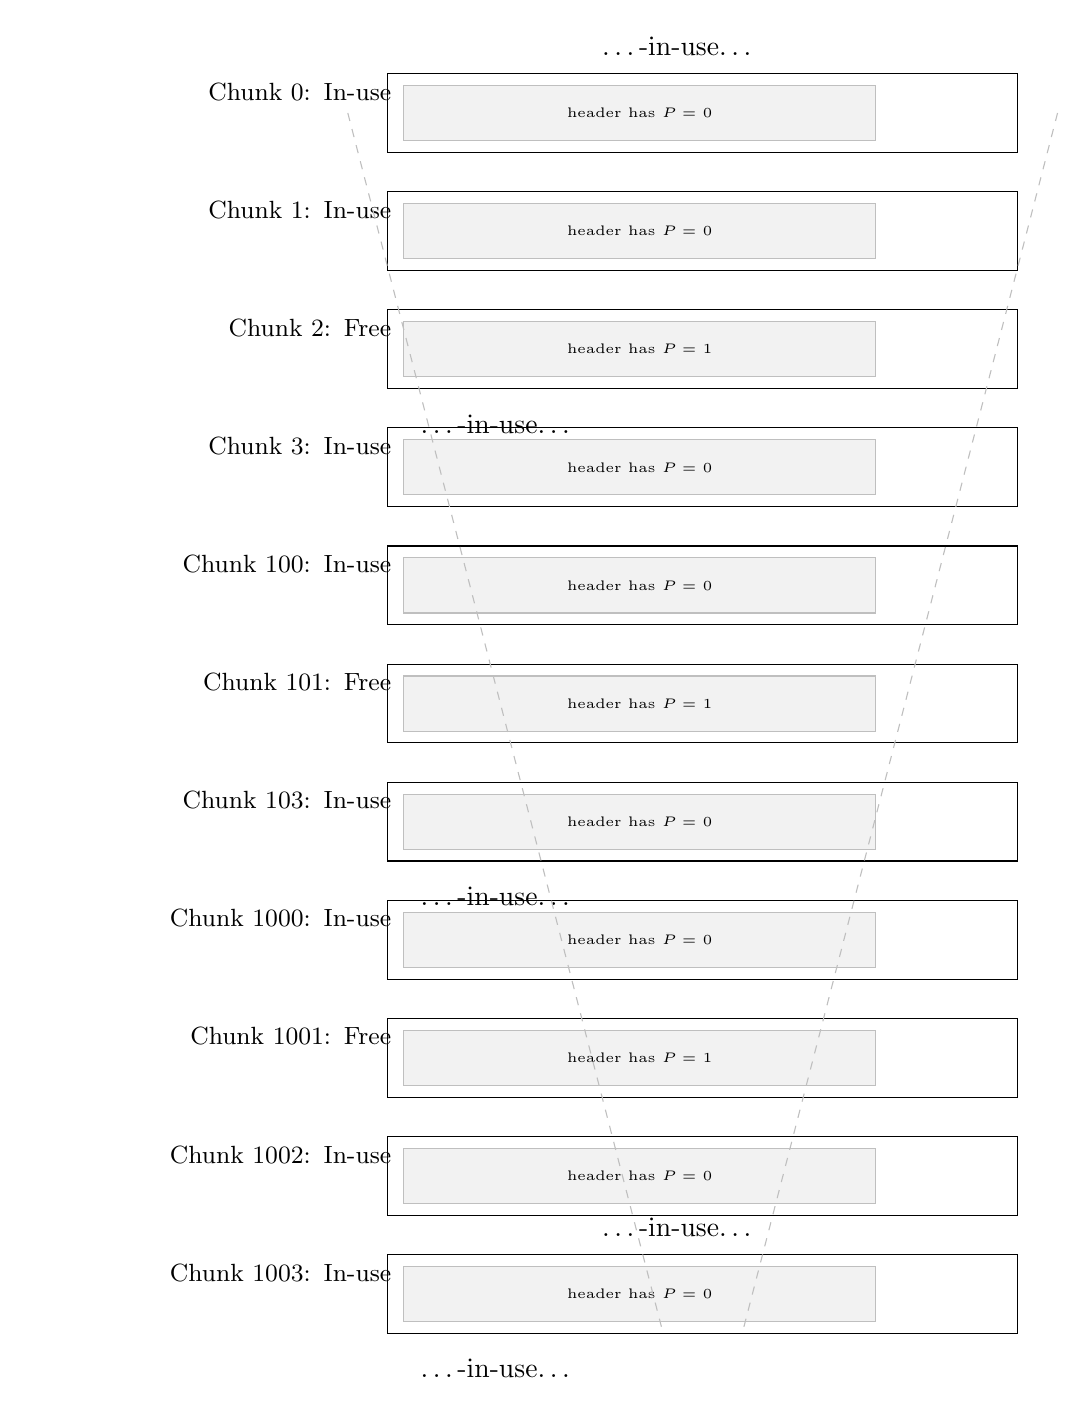
\begin{tikzpicture}[
    node distance=5pt,
    box/.style={
        draw,
        minimum width=8cm,
        minimum height=1cm,
        align=center,
        text depth=0ex,
        font=\small
    },
    header/.style={
        draw=gray!50,
        fill=gray!10,
        minimum width=6cm,
        minimum height=0.7cm,
        align=center,
        text depth=0ex,
        font=\footnotesize
    },
    label/.style={
        text width=4.5cm,
        align=right,
        font=\small
    }
]

% Define the chunks
\foreach \i/\status [count=\j from 0] in {
    0/In-use,
    1/In-use,
    2/Free,
    3/In-use,
    100/In-use,
    101/Free,
    103/In-use,
    1000/In-use,
    1001/Free,
    1002/In-use,
    1003/In-use
} {
    \node[box, name=chunk-\j] at (0,-\j*1.5) {};
    \node[label, right=of chunk-\j.north west, anchor=north east] {Chunk \i: \status};
    
    % Add the header inside each chunk
    \node[header, above right=0.15cm and 0.2cm of chunk-\j.south west, anchor=south west] 
        (header-\j) {\tiny header has $P=$ \ifnum\i=2 1\else\ifnum\i=101 1\else\ifnum\i=1001 1\else 0\fi\fi\fi};

    % Add content inside each chunk
    \ifnum\i=2
        \node[below=0.1cm of chunk-\j.south west, anchor=north west, xshift=0.3cm, yshift=-0.1cm] {\ldots-in-use\ldots};
    \else
        \ifnum\i=103
            \node[below=0.1cm of chunk-\j.south west, anchor=north west, xshift=0.3cm, yshift=-0.1cm] {\ldots-in-use\ldots};
        \else
            \ifnum\i=1003
                \node[below=0.1cm of chunk-\j.south west, anchor=north west, xshift=0.3cm, yshift=-0.1cm] {\ldots-in-use\ldots};
            \fi
        \fi
    \fi
}

% Draw dashed lines separating chunks
\draw[dashed, gray!50] ([xshift=-0.5cm]chunk-0.west) -- ([xshift=-0.5cm]chunk-10.south);
\draw[dashed, gray!50] ([xshift=0.5cm]chunk-0.east) -- ([xshift=0.5cm]chunk-10.south);

% Add top labels
\node[above=0.1cm of chunk-0.north, anchor=south, xshift=-0.3cm] {\ldots-in-use\ldots};
\node[above=0.1cm of chunk-10.north, anchor=south, xshift=-0.3cm] {\ldots-in-use\ldots};

\end{tikzpicture}

\end{document}